\documentclass[11pt, oneside]{article}   	% use "amsart" instead of "article" for AMSLaTeX format
\usepackage{geometry}                		% See geometry.pdf to learn the layout options. There are lots.
\geometry{letterpaper}                   		% ... or a4paper or a5paper or ... 
%\geometry{landscape}                		% Activate for for rotated page geometry
%\usepackage[parfill]{parskip}    		% Activate to begin paragraphs with an empty line rather than an indent
\usepackage{graphicx}				% Use pdf, png, jpg, or eps� with pdflatex; use eps in DVI mode
								% TeX will automatically convert eps --> pdf in pdflatex		
\usepackage{amssymb}
\usepackage{amsmath}
\usepackage{parskip}
\usepackage{color}

\title{Ellipse-parametrization}
%\author{The Author}
%\section{}
% \subsection*{R code}
\date{}							% Activate to display a given date or no date

\graphicspath{{/Users/telliott_admin/Dropbox/Tex/png/}}

% \begin{center} 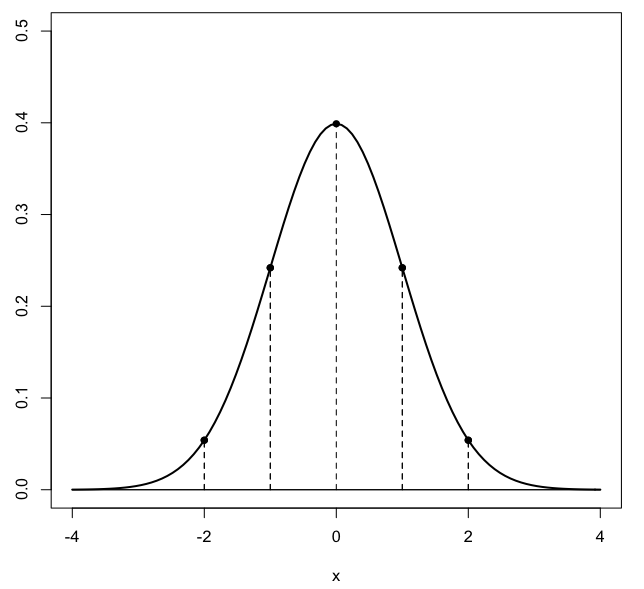
\includegraphics [scale=0.4] {gauss3.png} \end{center}
% \begin{bmatrix} a  &  b \\ c  &  d \end{bmatrix}
% \bigg |_

\begin{document}
\maketitle
\Large
%\noindent

\begin{center} 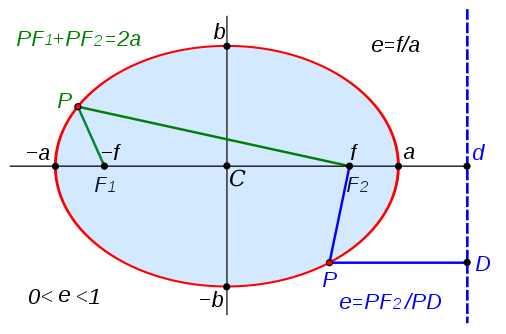
\includegraphics [scale=0.5] {ellipse_wikipedia.png} \end{center}

I want to compute the volume of an ellipsoid.  We imagine the solid formed by rotating the ellipse around the $x$-axis.  For each value of $x$, this solid will have a cross-section whose radius is equal to $y$, so to get the volume of the ellipse we do

\[ V = \int_{-a}^{a} \pi y^2 dx \]

Now, 
\[ x = a \cos t \]
\[ dx = -a \sin t \ dt \]
And we will have to find new limits for the integral.  Let's set it up first
So
\[ V = \pi \int (b^2 \sin^2 t)(-a \sin t) \ dt\]
Previously we had 
\[ x = -a \rightarrow a \]
The lower limit corresponds to $t = \pi$ and the upper limit to $t=0$.
\[ V = \pi a b^2 \int_{\pi}^{0} (\sin^2 t) (- \sin t) \ dt\]
\[ = \pi a b^2 \int_{\pi}^{0} (1 - \cos^2 t) (- \sin t) \ dt\]
\[ = \pi a b^2 \ [ \ \cos t - \frac{1}{3} cos^3 t \ ] \ \bigg |_{\pi}^{0} \]
\[ = \pi a b^2 \ [ \ (1 - \frac{1}{3}) - (-1 + \frac{1}{3})   \ ] \  \]
\[ = \frac{4}{3} \pi a b^2  \]

This is quite beautiful.  If we consider the three axes in space, for $y$ and $z$ the surface passes through at $b$, so $b$ counts twice in the volume.  If we rotated the other way (around the $y$ axis), we would obtain $\frac{4}{3} \pi a^2 b$.



\end{document}  